\documentclass[twoside]{book}

% Packages required by doxygen
\usepackage{calc}
\usepackage{doxygen}
\usepackage{graphicx}
\usepackage[utf8]{inputenc}
\usepackage{makeidx}
\usepackage{multicol}
\usepackage{multirow}
\usepackage{textcomp}
\usepackage[table]{xcolor}

% Font selection
\usepackage[T1]{fontenc}
\usepackage{mathptmx}
\usepackage[scaled=.90]{helvet}
\usepackage{courier}
\usepackage{amssymb}
\usepackage{sectsty}
\renewcommand{\familydefault}{\sfdefault}
\allsectionsfont{%
  \fontseries{bc}\selectfont%
  \color{darkgray}%
}
\renewcommand{\DoxyLabelFont}{%
  \fontseries{bc}\selectfont%
  \color{darkgray}%
}

% Page & text layout
\usepackage{geometry}
\geometry{%
  a4paper,%
  top=2.5cm,%
  bottom=2.5cm,%
  left=2.5cm,%
  right=2.5cm%
}
\tolerance=750
\hfuzz=15pt
\hbadness=750
\setlength{\emergencystretch}{15pt}
\setlength{\parindent}{0cm}
\setlength{\parskip}{0.2cm}
\makeatletter
\renewcommand{\paragraph}{%
  \@startsection{paragraph}{4}{0ex}{-1.0ex}{1.0ex}{%
    \normalfont\normalsize\bfseries\SS@parafont%
  }%
}
\renewcommand{\subparagraph}{%
  \@startsection{subparagraph}{5}{0ex}{-1.0ex}{1.0ex}{%
    \normalfont\normalsize\bfseries\SS@subparafont%
  }%
}
\makeatother

% Headers & footers
\usepackage{fancyhdr}
\pagestyle{fancyplain}
\fancyhead[LE]{\fancyplain{}{\bfseries\thepage}}
\fancyhead[CE]{\fancyplain{}{}}
\fancyhead[RE]{\fancyplain{}{\bfseries\leftmark}}
\fancyhead[LO]{\fancyplain{}{\bfseries\rightmark}}
\fancyhead[CO]{\fancyplain{}{}}
\fancyhead[RO]{\fancyplain{}{\bfseries\thepage}}
\fancyfoot[LE]{\fancyplain{}{}}
\fancyfoot[CE]{\fancyplain{}{}}
\fancyfoot[RE]{\fancyplain{}{\bfseries\scriptsize Generated on Thu May 2 2019 21\-:09\-:20 for Feature\-Rec by Doxygen }}
\fancyfoot[LO]{\fancyplain{}{\bfseries\scriptsize Generated on Thu May 2 2019 21\-:09\-:20 for Feature\-Rec by Doxygen }}
\fancyfoot[CO]{\fancyplain{}{}}
\fancyfoot[RO]{\fancyplain{}{}}
\renewcommand{\footrulewidth}{0.4pt}
\renewcommand{\chaptermark}[1]{%
  \markboth{#1}{}%
}
\renewcommand{\sectionmark}[1]{%
  \markright{\thesection\ #1}%
}

% Indices & bibliography
\usepackage{natbib}
\usepackage[titles]{tocloft}
\setcounter{tocdepth}{3}
\setcounter{secnumdepth}{5}
\makeindex

% Hyperlinks (required, but should be loaded last)
\usepackage{ifpdf}
\ifpdf
  \usepackage[pdftex,pagebackref=true]{hyperref}
\else
  \usepackage[ps2pdf,pagebackref=true]{hyperref}
\fi
\hypersetup{%
  colorlinks=true,%
  linkcolor=blue,%
  citecolor=blue,%
  unicode%
}

% Custom commands
\newcommand{\clearemptydoublepage}{%
  \newpage{\pagestyle{empty}\cleardoublepage}%
}


%===== C O N T E N T S =====

\begin{document}

% Titlepage & ToC
\hypersetup{pageanchor=false}
\pagenumbering{roman}
\begin{titlepage}
\vspace*{7cm}
\begin{center}%
{\Large Feature\-Rec }\\
\vspace*{1cm}
{\large Generated by Doxygen 1.8.5}\\
\vspace*{0.5cm}
{\small Thu May 2 2019 21:09:20}\\
\end{center}
\end{titlepage}
\clearemptydoublepage
\tableofcontents
\clearemptydoublepage
\pagenumbering{arabic}
\hypersetup{pageanchor=true}

%--- Begin generated contents ---
\chapter{Hierarchical Index}
\section{Class Hierarchy}
This inheritance list is sorted roughly, but not completely, alphabetically\-:\begin{DoxyCompactList}
\item \contentsline{section}{Model\-Edge}{\pageref{classModelEdge}}{}
\item Topo\-D\-S\-\_\-\-Face\begin{DoxyCompactList}
\item \contentsline{section}{Model\-Face}{\pageref{classModelFace}}{}
\begin{DoxyCompactList}
\item \contentsline{section}{Bend}{\pageref{classBend}}{}
\end{DoxyCompactList}
\end{DoxyCompactList}
\end{DoxyCompactList}

\chapter{Class Index}
\section{Class List}
Here are the classes, structs, unions and interfaces with brief descriptions\-:\begin{DoxyCompactList}
\item\contentsline{section}{\hyperlink{classBend}{Bend} }{\pageref{classBend}}{}
\item\contentsline{section}{\hyperlink{classModelEdge}{Model\-Edge} }{\pageref{classModelEdge}}{}
\item\contentsline{section}{\hyperlink{classModelFace}{Model\-Face} }{\pageref{classModelFace}}{}
\end{DoxyCompactList}

\chapter{Class Documentation}
\hypertarget{classBend}{\section{Bend Class Reference}
\label{classBend}\index{Bend@{Bend}}
}
Inheritance diagram for Bend\-:\begin{figure}[H]
\begin{center}
\leavevmode
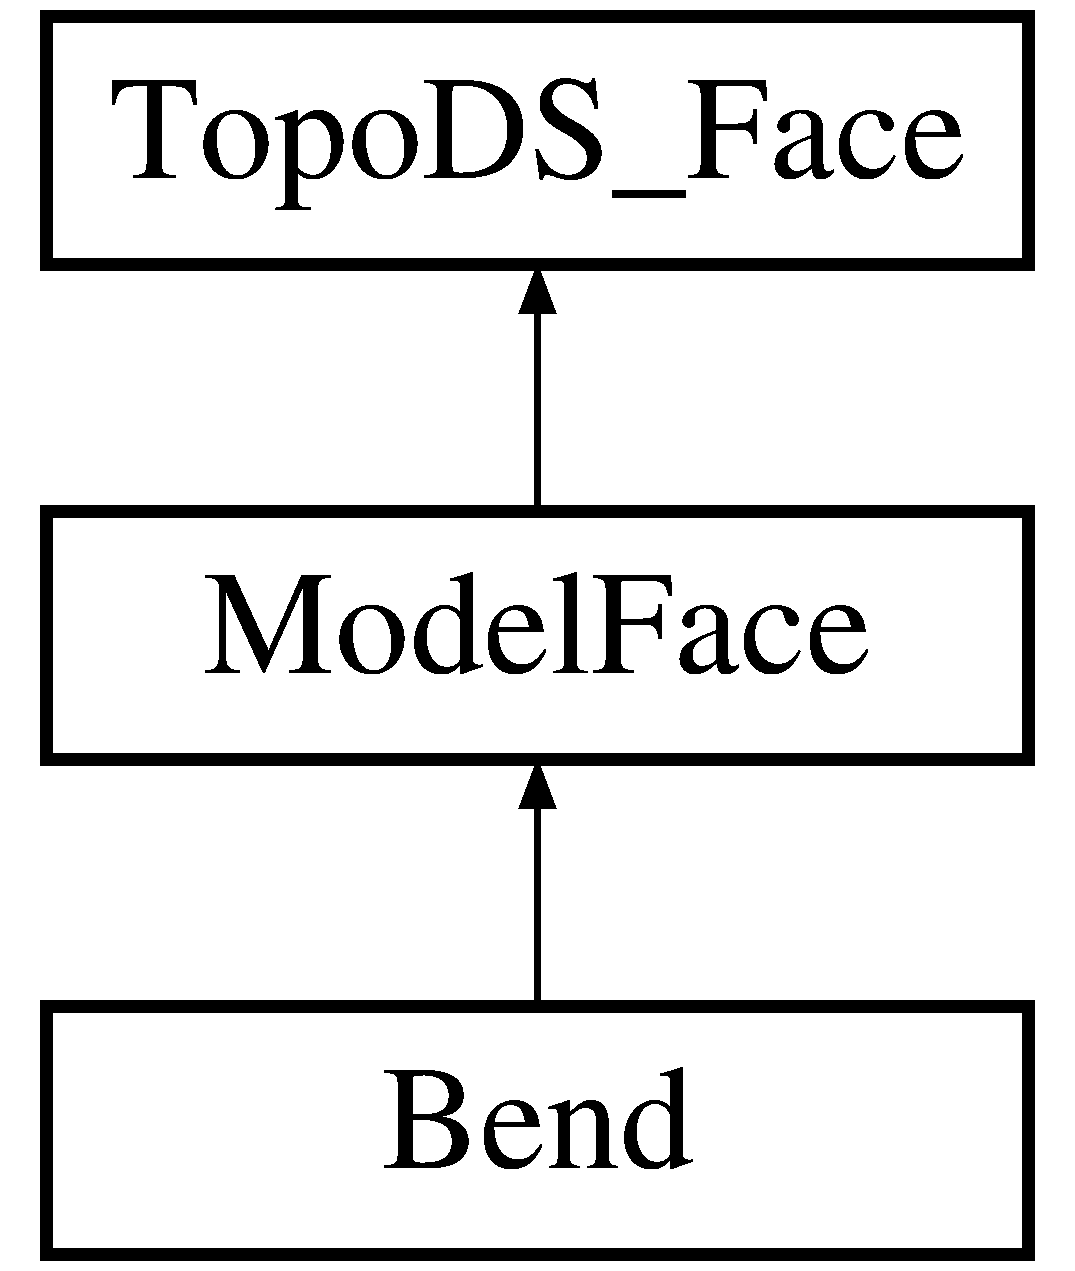
\includegraphics[height=3.000000cm]{classBend}
\end{center}
\end{figure}
\subsection*{Additional Inherited Members}


The documentation for this class was generated from the following file\-:\begin{DoxyCompactItemize}
\item 
bend.\-h\end{DoxyCompactItemize}

\hypertarget{classModelEdge}{\section{Model\-Edge Class Reference}
\label{classModelEdge}\index{Model\-Edge@{Model\-Edge}}
}
\subsection*{Public Member Functions}
\begin{DoxyCompactItemize}
\item 
\hypertarget{classModelEdge_a0663679e1a3462593bb2cec05f8a052f}{{\bfseries Model\-Edge} (gp\-\_\-\-Pnt startv\mbox{[}$\,$\mbox{]})}\label{classModelEdge_a0663679e1a3462593bb2cec05f8a052f}

\item 
\hypertarget{classModelEdge_a953b7fcf296b5dd3703780baf0ded2be}{void {\bfseries set\-Is\-Rational} (bool is\-\_\-it)}\label{classModelEdge_a953b7fcf296b5dd3703780baf0ded2be}

\item 
\hypertarget{classModelEdge_af452e2f9b781288175da8e8fc6a6b3b6}{bool {\bfseries Is\-Rational} ()}\label{classModelEdge_af452e2f9b781288175da8e8fc6a6b3b6}

\item 
\hypertarget{classModelEdge_a42f6669f57658d404afbfdabc3785078}{void {\bfseries set\-Edge\-Num} (Standard\-\_\-\-Integer enumb)}\label{classModelEdge_a42f6669f57658d404afbfdabc3785078}

\item 
\hypertarget{classModelEdge_ac4165c644c04eb07e00319fdcab4badf}{Standard\-\_\-\-Integer {\bfseries get\-Edge\-Num} () const }\label{classModelEdge_ac4165c644c04eb07e00319fdcab4badf}

\item 
\hypertarget{classModelEdge_a2e938d40d28bf46e21cf536fd79ec534}{void {\bfseries set\-Edge\-Type} (Edge\-Type etype)}\label{classModelEdge_a2e938d40d28bf46e21cf536fd79ec534}

\item 
\hypertarget{classModelEdge_a5acee2e41d8937d2634b4df9983740c5}{Edge\-Type {\bfseries get\-Edge\-Type} ()}\label{classModelEdge_a5acee2e41d8937d2634b4df9983740c5}

\item 
\hypertarget{classModelEdge_aff4e68680c30a39f581adb5691d44148}{void {\bfseries set\-Edge\-Position} (Edge\-Position epos)}\label{classModelEdge_aff4e68680c30a39f581adb5691d44148}

\item 
\hypertarget{classModelEdge_ab32f96c247c6c5b9ca32928a4b05132b}{Edge\-Position {\bfseries get\-Edge\-Position} ()}\label{classModelEdge_ab32f96c247c6c5b9ca32928a4b05132b}

\item 
\hypertarget{classModelEdge_a970fbeef1a1fd83b0d3dfa7bbcf40530}{void {\bfseries set\-Edge\-Length} (Standard\-\_\-\-Real len)}\label{classModelEdge_a970fbeef1a1fd83b0d3dfa7bbcf40530}

\item 
\hypertarget{classModelEdge_a7bc299ce1147f406905ac89f961632f9}{Standard\-\_\-\-Real {\bfseries get\-Edge\-Length} ()}\label{classModelEdge_a7bc299ce1147f406905ac89f961632f9}

\item 
\hypertarget{classModelEdge_a4116750cf19e091acff7b5ca910f221e}{void {\bfseries set\-Line\-Vector} (gp\-\_\-\-Pnt l\-\_\-vector)}\label{classModelEdge_a4116750cf19e091acff7b5ca910f221e}

\item 
\hypertarget{classModelEdge_a7274e0ba97408832fceaabd9fdcc13f1}{gp\-\_\-\-Pnt {\bfseries get\-Line\-Vector} ()}\label{classModelEdge_a7274e0ba97408832fceaabd9fdcc13f1}

\item 
\hypertarget{classModelEdge_abd033ecdc2b7bdcad613188cfb0f3349}{void {\bfseries set\-Line\-Unit\-Vector} (gp\-\_\-\-Pnt lu\-\_\-vector)}\label{classModelEdge_abd033ecdc2b7bdcad613188cfb0f3349}

\item 
\hypertarget{classModelEdge_a8a5ae73ed6c60758d80c6cff4a418137}{gp\-\_\-\-Pnt {\bfseries get\-Line\-Unit\-Vector} ()}\label{classModelEdge_a8a5ae73ed6c60758d80c6cff4a418137}

\end{DoxyCompactItemize}
\subsection*{Static Public Member Functions}
\begin{DoxyCompactItemize}
\item 
\hypertarget{classModelEdge_a5a99dd41b668434d6dc820f6a2132616}{static bool {\bfseries compare\-\_\-edges} (\hyperlink{classModelEdge}{Model\-Edge} edge1, \hyperlink{classModelEdge}{Model\-Edge} edge2)}\label{classModelEdge_a5a99dd41b668434d6dc820f6a2132616}

\item 
\hypertarget{classModelEdge_a238b22538e45c99a2377a9b31c25aff2}{static bool {\bfseries compare\-\_\-vl} (gp\-\_\-\-Pnt v1, gp\-\_\-\-Pnt v2)}\label{classModelEdge_a238b22538e45c99a2377a9b31c25aff2}

\end{DoxyCompactItemize}
\subsection*{Public Attributes}
\begin{DoxyCompactItemize}
\item 
\hypertarget{classModelEdge_a16c9c6d7fed7e4b605af19d75303b49f}{int {\bfseries count}}\label{classModelEdge_a16c9c6d7fed7e4b605af19d75303b49f}

\item 
\hypertarget{classModelEdge_a2b3178c1328aab725d2b788944ba59eb}{Standard\-\_\-\-Integer {\bfseries edge\-\_\-number}}\label{classModelEdge_a2b3178c1328aab725d2b788944ba59eb}

\item 
\hypertarget{classModelEdge_ace75c9b1b2a9f48687a706cecdcd6421}{Edge\-Type {\bfseries edge\-\_\-type}}\label{classModelEdge_ace75c9b1b2a9f48687a706cecdcd6421}

\item 
\hypertarget{classModelEdge_a84288312bd23387a2e58dafbccba747a}{Edge\-Position {\bfseries edge\-\_\-position}}\label{classModelEdge_a84288312bd23387a2e58dafbccba747a}

\item 
\hypertarget{classModelEdge_a7f84cbd7c08233e9bff4daf5fef6e2f2}{gp\-\_\-\-Pnt {\bfseries line\-\_\-vector}}\label{classModelEdge_a7f84cbd7c08233e9bff4daf5fef6e2f2}

\item 
\hypertarget{classModelEdge_a6781992388ba080fa9587e333d7e7175}{gp\-\_\-\-Pnt {\bfseries line\-\_\-unit\-\_\-vector}}\label{classModelEdge_a6781992388ba080fa9587e333d7e7175}

\item 
\hypertarget{classModelEdge_a8773f669ad2b8a4f48ba4e021eaada46}{gp\-\_\-\-Pnt {\bfseries start\-\_\-vertex}}\label{classModelEdge_a8773f669ad2b8a4f48ba4e021eaada46}

\item 
\hypertarget{classModelEdge_a12c482570889cdbb3ec93f8c1bade66b}{gp\-\_\-\-Pnt {\bfseries terminate\-\_\-vertex}}\label{classModelEdge_a12c482570889cdbb3ec93f8c1bade66b}

\item 
\hypertarget{classModelEdge_ac4bbc24ad8305422b45c30cd4044d46f}{Standard\-\_\-\-Real {\bfseries edge\-\_\-length}}\label{classModelEdge_ac4bbc24ad8305422b45c30cd4044d46f}

\item 
\hypertarget{classModelEdge_a8d846f8085eb4cc662932a930472585a}{bool {\bfseries isrational}}\label{classModelEdge_a8d846f8085eb4cc662932a930472585a}

\item 
\hypertarget{classModelEdge_a5a0a8c9fdb9463e0aeb9cf98631c5665}{Standard\-\_\-\-Integer {\bfseries same\-\_\-as\-\_\-edge\-\_\-number}}\label{classModelEdge_a5a0a8c9fdb9463e0aeb9cf98631c5665}

\end{DoxyCompactItemize}


The documentation for this class was generated from the following file\-:\begin{DoxyCompactItemize}
\item 
Model\-Edge.\-h\end{DoxyCompactItemize}

\hypertarget{classModelFace}{\section{Model\-Face Class Reference}
\label{classModelFace}\index{Model\-Face@{Model\-Face}}
}


{\ttfamily \#include $<$Model\-Face.\-h$>$}

Inheritance diagram for Model\-Face\-:\begin{figure}[H]
\begin{center}
\leavevmode
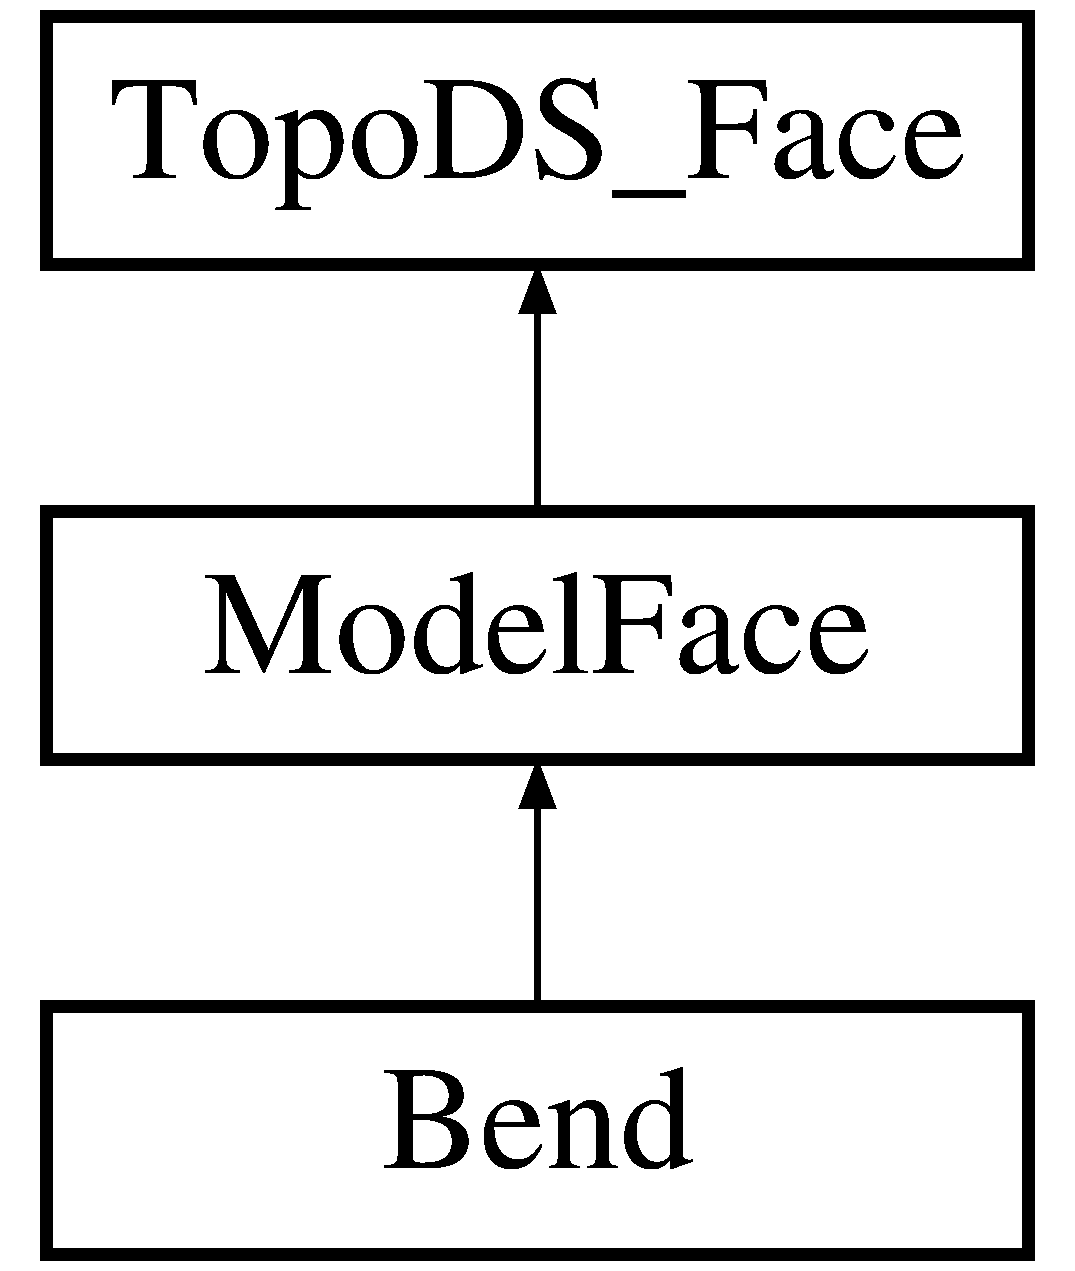
\includegraphics[height=3.000000cm]{classModelFace}
\end{center}
\end{figure}
\subsection*{Public Member Functions}
\begin{DoxyCompactItemize}
\item 
\hypertarget{classModelFace_a63cefab86b4dfec7caac9a9d8abc0c07}{void {\bfseries set\-Joining\-Face\-I\-D1} (Standard\-\_\-\-Integer face\-\_\-id)}\label{classModelFace_a63cefab86b4dfec7caac9a9d8abc0c07}

\item 
\hypertarget{classModelFace_a6e3135935eac6d20013e9a7f6b5d7492}{Standard\-\_\-\-Integer {\bfseries get\-Joining\-Face\-I\-D1} ()}\label{classModelFace_a6e3135935eac6d20013e9a7f6b5d7492}

\item 
\hypertarget{classModelFace_a55c2af23e5b4fef4532996560b71f76f}{void {\bfseries set\-Joining\-Face\-I\-D2} (Standard\-\_\-\-Integer face\-\_\-id)}\label{classModelFace_a55c2af23e5b4fef4532996560b71f76f}

\item 
\hypertarget{classModelFace_a0266a6e805ace7ea414da2a4c1e13975}{Standard\-\_\-\-Integer {\bfseries get\-Joining\-Face\-I\-D2} ()}\label{classModelFace_a0266a6e805ace7ea414da2a4c1e13975}

\item 
void \hyperlink{classModelFace_acbf209155f59f95036935dd082281aa8}{set\-Curvature} (Standard\-\_\-\-Real cv)
\item 
\hypertarget{classModelFace_aaf6871e0fdb9b9cd07745cb39b5b816b}{Standard\-\_\-\-Real {\bfseries get\-Face\-Radius} ()}\label{classModelFace_aaf6871e0fdb9b9cd07745cb39b5b816b}

\item 
\hypertarget{classModelFace_a0984a9f0ded1a02949c4b7bc93348f14}{void {\bfseries set\-Face\-Id} (Standard\-\_\-\-Integer fid)}\label{classModelFace_a0984a9f0ded1a02949c4b7bc93348f14}

\item 
\hypertarget{classModelFace_afd47dfaca9c38b5e788edcfc705fcc43}{Standard\-\_\-\-Integer {\bfseries get\-Face\-Id} ()}\label{classModelFace_afd47dfaca9c38b5e788edcfc705fcc43}

\item 
\hypertarget{classModelFace_ae28293e19bdb459edbf4322ac2d3cf70}{void {\bfseries set\-Unit\-Normal} (gp\-\_\-\-Dir unit\-\_\-normal)}\label{classModelFace_ae28293e19bdb459edbf4322ac2d3cf70}

\item 
void \hyperlink{classModelFace_ac6d00879fc8784039db1cd303326f18a}{compute\-Face\-Equation} ()
\item 
\hypertarget{classModelFace_a30b9802b65ad3db53121d4da7215e0e9}{gp\-\_\-\-Pnt {\bfseries get\-Face\-Normal} ()}\label{classModelFace_a30b9802b65ad3db53121d4da7215e0e9}

\item 
\hypertarget{classModelFace_a11e3cf3a4eae9a30e59c37669fecf003}{void {\bfseries set\-Face\-Type} (Face\-Type ftype)}\label{classModelFace_a11e3cf3a4eae9a30e59c37669fecf003}

\item 
\hypertarget{classModelFace_acf740712dfb0d9583b4d9f3f501e2ebc}{Face\-Type {\bfseries get\-Face\-Type} ()}\label{classModelFace_acf740712dfb0d9583b4d9f3f501e2ebc}

\item 
\hypertarget{classModelFace_a801dcaeed2a3079d1f168eba1ff2fa9b}{void {\bfseries set\-Plane\-Type} (Plane\-Type ptype)}\label{classModelFace_a801dcaeed2a3079d1f168eba1ff2fa9b}

\item 
\hypertarget{classModelFace_ae1959b248ed0a313ea20da30d5745c87}{Plane\-Type {\bfseries get\-Plane\-Type} ()}\label{classModelFace_ae1959b248ed0a313ea20da30d5745c87}

\item 
void \hyperlink{classModelFace_aa3be5b689b9a58787237b3796be24b71}{print\-Unit\-Normal} ()
\item 
\hypertarget{classModelFace_af2be0135b073a01349a740e1a5f53ba7}{void {\bfseries add\-Edge} (const \hyperlink{classModelEdge}{Model\-Edge} \&n)}\label{classModelFace_af2be0135b073a01349a740e1a5f53ba7}

\item 
\hypertarget{classModelFace_a320c3f19bef69664d9157f8b641b9f82}{std\-::vector$<$ \hyperlink{classModelEdge}{Model\-Edge} $>$ {\bfseries get\-Face\-Edges} ()}\label{classModelFace_a320c3f19bef69664d9157f8b641b9f82}

\item 
void \hyperlink{classModelFace_a68807415019fb1e6bf38d779b34fc3bb}{compute\-Face\-Normal} ()
\end{DoxyCompactItemize}
\subsection*{Static Public Member Functions}
\begin{DoxyCompactItemize}
\item 
static void \hyperlink{classModelFace_a0b3dcbc372588a50785e2252fedcfab2}{classify\-Edges} (std\-::vector$<$ \hyperlink{classModelFace}{Model\-Face} $>$ \&faces)
\item 
static void \hyperlink{classModelFace_a239a33e0969b8b740f7dcb0b26a7aebd}{classify\-B\-S\-\_\-\-B\-F} (std\-::vector$<$ \hyperlink{classModelFace}{Model\-Face} $>$ \&faces)
\item 
static void \hyperlink{classModelFace_a787db625e224903c894808c8aed7056b}{classify\-Faces} (std\-::vector$<$ \hyperlink{classModelFace}{Model\-Face} $>$ \&faces)
\end{DoxyCompactItemize}


\subsection{Detailed Description}
This class describes a face of a model shape. It inherits from the Open\-Cascade Topo\-D\-S\-\_\-\-Face class.

\begin{DoxyNote}{Note}
Attempts at zen rarely work.
\end{DoxyNote}
\begin{DoxyAuthor}{Author}
(last to touch it) 
\end{DoxyAuthor}
\begin{DoxyParagraph}{Author\-:}
Wilfred Dube 
\end{DoxyParagraph}


\begin{DoxyVersion}{Version}

\end{DoxyVersion}
\begin{DoxyParagraph}{Revision\-:}
1.\-0 
\end{DoxyParagraph}


\begin{DoxyDate}{Date}

\end{DoxyDate}
\begin{DoxyParagraph}{Date\-:}
2019/05/02 14\-:16\-:20 
\end{DoxyParagraph}


Contact\-: \href{mailto:wilfreddube@gmail.com}{\tt wilfreddube@gmail.\-com}

Created on\-: Wed Apr 10 18\-:39\-:37 2019 

\subsection{Member Function Documentation}
\hypertarget{classModelFace_a239a33e0969b8b740f7dcb0b26a7aebd}{\index{Model\-Face@{Model\-Face}!classify\-B\-S\-\_\-\-B\-F@{classify\-B\-S\-\_\-\-B\-F}}
\index{classify\-B\-S\-\_\-\-B\-F@{classify\-B\-S\-\_\-\-B\-F}!ModelFace@{Model\-Face}}
\subsubsection[{classify\-B\-S\-\_\-\-B\-F}]{\setlength{\rightskip}{0pt plus 5cm}static void Model\-Face\-::classify\-B\-S\-\_\-\-B\-F (
\begin{DoxyParamCaption}
\item[{std\-::vector$<$ {\bf Model\-Face} $>$ \&}]{faces}
\end{DoxyParamCaption}
)\hspace{0.3cm}{\ttfamily [inline]}, {\ttfamily [static]}}}\label{classModelFace_a239a33e0969b8b740f7dcb0b26a7aebd}
Identifies B\-E\-N\-D\-\_\-\-F\-A\-C\-E and B\-E\-N\-D\-\_\-\-S\-I\-D\-E faces types. 
\begin{DoxyParams}{Parameters}
{\em faces} & a list for faces. \\
\hline
\end{DoxyParams}
\hypertarget{classModelFace_a0b3dcbc372588a50785e2252fedcfab2}{\index{Model\-Face@{Model\-Face}!classify\-Edges@{classify\-Edges}}
\index{classify\-Edges@{classify\-Edges}!ModelFace@{Model\-Face}}
\subsubsection[{classify\-Edges}]{\setlength{\rightskip}{0pt plus 5cm}static void Model\-Face\-::classify\-Edges (
\begin{DoxyParamCaption}
\item[{std\-::vector$<$ {\bf Model\-Face} $>$ \&}]{faces}
\end{DoxyParamCaption}
)\hspace{0.3cm}{\ttfamily [inline]}, {\ttfamily [static]}}}\label{classModelFace_a0b3dcbc372588a50785e2252fedcfab2}
Classifies the edges in each face based on whether they are rational or polynomial (A\-R\-C or S\-T\-R\-A\-I\-G\-H\-T\-\_\-\-L\-I\-N\-E). 
\begin{DoxyParams}{Parameters}
{\em faces} & a list for faces. \\
\hline
\end{DoxyParams}
\hypertarget{classModelFace_a787db625e224903c894808c8aed7056b}{\index{Model\-Face@{Model\-Face}!classify\-Faces@{classify\-Faces}}
\index{classify\-Faces@{classify\-Faces}!ModelFace@{Model\-Face}}
\subsubsection[{classify\-Faces}]{\setlength{\rightskip}{0pt plus 5cm}static void Model\-Face\-::classify\-Faces (
\begin{DoxyParamCaption}
\item[{std\-::vector$<$ {\bf Model\-Face} $>$ \&}]{faces}
\end{DoxyParamCaption}
)\hspace{0.3cm}{\ttfamily [inline]}, {\ttfamily [static]}}}\label{classModelFace_a787db625e224903c894808c8aed7056b}
Identifies F\-A\-C\-E and T\-H\-I\-C\-K\-N\-E\-S\-S\-\_\-\-D\-E\-F\-I\-N\-I\-N\-G\-\_\-\-F\-A\-C\-E faces types. Retrieves the B\-E\-N\-D\-\_\-\-F\-A\-C\-E type faces and compares its S\-T\-R\-A\-I\-G\-H\-T\-\_\-\-L\-I\-N\-E edge type edge to all the P\-L\-A\-N\-A\-R type face. If there is a matching edge then the bend is connected to that face. The joining face I\-D is set to the connected face's I\-D. The connected face's Face\-Type is also set to F\-A\-C\-E. 
\begin{DoxyParams}{Parameters}
{\em faces} & a list for faces. \\
\hline
\end{DoxyParams}
\hypertarget{classModelFace_ac6d00879fc8784039db1cd303326f18a}{\index{Model\-Face@{Model\-Face}!compute\-Face\-Equation@{compute\-Face\-Equation}}
\index{compute\-Face\-Equation@{compute\-Face\-Equation}!ModelFace@{Model\-Face}}
\subsubsection[{compute\-Face\-Equation}]{\setlength{\rightskip}{0pt plus 5cm}void Model\-Face\-::compute\-Face\-Equation (
\begin{DoxyParamCaption}
{}
\end{DoxyParamCaption}
)\hspace{0.3cm}{\ttfamily [inline]}}}\label{classModelFace_ac6d00879fc8784039db1cd303326f18a}
calculates and sets the D value of the equation of a plane (Ax+\-By+\-Cz = D). \hypertarget{classModelFace_a68807415019fb1e6bf38d779b34fc3bb}{\index{Model\-Face@{Model\-Face}!compute\-Face\-Normal@{compute\-Face\-Normal}}
\index{compute\-Face\-Normal@{compute\-Face\-Normal}!ModelFace@{Model\-Face}}
\subsubsection[{compute\-Face\-Normal}]{\setlength{\rightskip}{0pt plus 5cm}void Model\-Face\-::compute\-Face\-Normal (
\begin{DoxyParamCaption}
{}
\end{DoxyParamCaption}
)\hspace{0.3cm}{\ttfamily [inline]}}}\label{classModelFace_a68807415019fb1e6bf38d779b34fc3bb}
computes and sets the normal vector of the face. \hypertarget{classModelFace_aa3be5b689b9a58787237b3796be24b71}{\index{Model\-Face@{Model\-Face}!print\-Unit\-Normal@{print\-Unit\-Normal}}
\index{print\-Unit\-Normal@{print\-Unit\-Normal}!ModelFace@{Model\-Face}}
\subsubsection[{print\-Unit\-Normal}]{\setlength{\rightskip}{0pt plus 5cm}void Model\-Face\-::print\-Unit\-Normal (
\begin{DoxyParamCaption}
{}
\end{DoxyParamCaption}
)\hspace{0.3cm}{\ttfamily [inline]}}}\label{classModelFace_aa3be5b689b9a58787237b3796be24b71}
prints out the unit normal vector of the face. \hypertarget{classModelFace_acbf209155f59f95036935dd082281aa8}{\index{Model\-Face@{Model\-Face}!set\-Curvature@{set\-Curvature}}
\index{set\-Curvature@{set\-Curvature}!ModelFace@{Model\-Face}}
\subsubsection[{set\-Curvature}]{\setlength{\rightskip}{0pt plus 5cm}void Model\-Face\-::set\-Curvature (
\begin{DoxyParamCaption}
\item[{Standard\-\_\-\-Real}]{cv}
\end{DoxyParamCaption}
)\hspace{0.3cm}{\ttfamily [inline]}}}\label{classModelFace_acbf209155f59f95036935dd082281aa8}
a normal member taking one argument to set the curvature attribute of the face. If the curvature != 0 then the face is a bend face and so its radius is also set. $\ast$ 
\begin{DoxyParams}{Parameters}
{\em cv} & a real/floating point. \\
\hline
\end{DoxyParams}


The documentation for this class was generated from the following file\-:\begin{DoxyCompactItemize}
\item 
Model\-Face.\-h\end{DoxyCompactItemize}

%--- End generated contents ---

% Index
\newpage
\phantomsection
\addcontentsline{toc}{part}{Index}
\printindex

\end{document}
